\documentclass[12pt,fleqn]{article}
\setlength{\parindent}{0pt}
\usepackage{graphicx}
\usepackage{listings}
\usepackage[latin5]{inputenc}
\setlength{\parskip}{8pt}
\setlength{\parsep}{0pt}
\setlength{\headsep}{0pt}
\setlength{\topskip}{0pt}
\setlength{\topmargin}{0pt}
\setlength{\topsep}{0pt}
\setlength{\partopsep}{0pt}
\setlength{\mathindent}{0cm}

\begin{document}
MIT OCW Cok Degiskenli Calculus - Ders 6

Bir onceki derste cycloid konusunu isledik. 

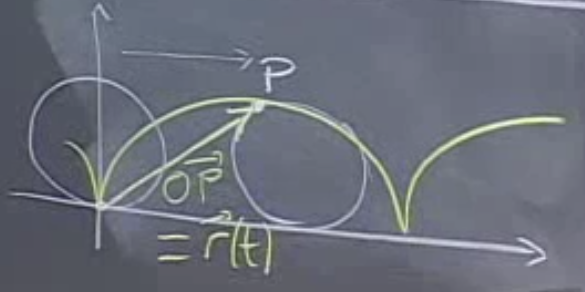
\includegraphics[height=4cm]{6_1.png}

Hareket eden bir noktanin pozisyonu

\[ (x(t), y(t), z(t)) \]

Bu noktayi takip etmenin diger yollarindan biri onu pozisyonu vektoru
olarak gormek, ki bu vektorun bilesenleri noktanin kordinatlari. 

\[ \vec{r}(t) = <x(t),y(t),z(t)> \]

Vektor orijin (baslangic) noktasindan gelinen noktayi isaret eden bir
vektor (resimde $\vec{OP}$). 

Cycloid probleminde tekerlek yaricapini 1 alalim ve birim hizda ilerliyor
olalim, ki boylece aci $\theta$ ve zaman ayni sey haline gelsin

\[ \vec{r}(t) = <t-sin(t), 1-cos(t) \]

Tamam. Simdi, noktanin pozisyonunu zaman acisindan bildigimize gore, onun
degisimini inceleyebiliriz, mesela hizina, ivmesine bakabiliriz. Ilk once
hiza bakabiliriz. Fakat, aslinda, hizdan daha iyisini hesaplayabiliriz. Hiz
tek bir sayidir sadece, ama eger su icinde GPS olan satafatli spor
arabalarindan birine sahip degilseniz, size hizinizin ``hangi yonde''
oldugunu soylemez. Sadece ``gittiginiz yonde'' (her ne yone gidiyorsaniz)
ne kadar hizli oldugunuzu soyler.

O zaman biz hizimizi hesaplarken, hem yonu, hem hizi ayni anda goze
alabiliriz. Bu demektir ki vektor kavrami tekrar isimize yarayacak. Hizi
vektor olarak hesaplayabiliriz. 

Bunu nasil yapariz? Pozisyon vektorunun zamana gore turevini alabiliriz.

\[ \vec{v} = \frac{d\vec{r}}{dt} \]

Bu tur bir turevi bu derste ilk kez goruyoruz, ilk kez bir vektorun
turevini aliyoruz. Bu sekilde turev almak demek, o vektorun bilesenlerinin
teker teker turevini almak demektir. Yani

\[ =
<\frac{dx}{dt}, \frac{dy}{dt}, \frac{dz}{dt}>
\]


Cycloid ornegine donersek

\[ \vec{r}(t) = <t-sin(t), 1-cos(t) \]

formulunun turevini alirsak ne olur? 

\[ \vec{v} = \frac{d\vec{r}}{dt} = <1-cos(t),sin(t)>\]

Iste bu turev bize hangi yonde ve ne kadar hizli gittigimizi gosteriyor. 

Bu arada bir vektorunun buyuklugunun (magnitude) her zaman mesafesel,
uzakliksal anlami olmayabilecegini de gormus oluyoruz. Hiz kavrami bir
orandir, katedilmis bir mesafe, bir yer degildir, $t$ aninda bir yonde olan
bir buyukluktur. Fakat yine de bir buyukluktur, bir yonu vardir, ve bu
sebeple vektorler ile temsil edilebilir. 

Problemimize donelim. Onceki derste tekerlekte izlenen noktanin en alta gelip
yukseldigi siralarda hareketinin nasil oldugunu irdelemistik. Simdi bu
konuyu hiz kavramini kullanarak incelemeye ugrasalim. Ustteki vektore $t=0$
koyarsam, ne olur? Sonuc $<0,0>$, yani $\vec{v} = 0$. Tabii ki nokta $t=0$
oncesi hareket ediyor, sonra da ediyor, yani bir hizi var, sadece ``o
anda'' hizi yok. 

Peki hiz vektor olarak daha fazla bilgi veriyor olmasina ragmen, ben yine
de klasik anlamda hizi, yani o tek sayiyi elde etmek istiyorsam ne yaparim?
Hiz vektorunun buyuklugunu hesaplarim, $|\vec{v}|$. 

\[ |\vec{v}| = \sqrt{ (1-cos(t))^2 + sin^2(t) } \]


\[ = \sqrt{ 1-2cos(t) + cos^2(t) + sin^2(t)  } \]


\[ = \sqrt{ 2-2cos(t) } \]


Bu formule bakarak hizin nerede en fazla, en az oldugunu
hesaplayabiliriz. Eger $t=0$ ise, sonuc sifir olur. $t=\pi$ ise elimizde
$\sqrt{4} = 2$ vardir, bu an noktanin tekerlegin en ustunde oldugu andir,
bu an ayni zamanda en hizli hareket ettigimiz de andir. Hatta bu hiz
tekerlegin saga dogru yatay gidis hizinin iki katidir, tekerlegin saga
dogru birim hizda ilerledigini soylemistik, fakat nokta bunun ustune bir de
merkeze gore bir donme hareketi icinde, ve bu iki etki birbirine eklenerek
$2$ hizina sebebiyet veriyor.

O nokta tepe noktasindan asagi inmeye baslayinca tabii ki noktamiz donusun
``geriye dogru'' olan etkisiyle toplami hizinda dusme yasiyor.

Ivme

Bu konuyu islemeden once klasik olarak bilinen ivme kavrami ile burada
kullanacagimiz ivme kavrami ile ciddi uyusmazliklar oldugunu
belirtmeliyim. Klasik anlayista ivme mesela bir arabada giderken
``hissettigimiz sey'' bizi koltuga iten kuvvet, hizdaki degisim (hizin
turevi) olarak bilinir, ve eger bir arabada saatte 40 km ile gidiyorsam,
ivme yok denir. Fakat simdi bu arabanin bir virajdan dondugunu farzedelim,
bu durumda bir kuvvet hissederiz, hala saatte 40 ile gidiyor olabilirim,
ama bir ivme vardir. Burada aslinda yana dogru bir hizlanma / ivme
sozkonusudur. O zaman yine vektor kavramini kullanmamiz lazim. 

Ivme vektorunu soyle belirtelim:

\[ \vec{a} = \frac{d\vec{v}}{dt} \]

Fizikteki ivme tanimi da budur, $F = ma$ derken kastedilen $a$ iste bu
$a$'dir. Bir vektordur. 

Cycloid'e donelim. 

\[ \vec{v} = <1-cos(t),sin(t)>\]

Turevi alalim

\[ \frac{d\vec{v}}{dt} = <sin(t), cos(t)>\]

$t=0$ noktasinda ivme nedir? $<0,1>$. 

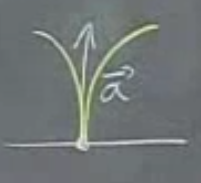
\includegraphics[height=3cm]{6_2.png}

Yani $t=0$ anindaki ivme bir birim vektor, ve yonu tam yukariya dogru. Bu
ilginc bir sey, o anda hiz sifir, fakat bir ivme mevcut. 

Bu arada, hemen belirtelim

\[ \bigg|\frac{d\vec{r}}{dt}\bigg|  \ne \frac{d|\vec{r}|}{dt}\]


Yani bir vektorun turevinin buyuklugu, o vektorun buyuklugunun turevi ile
ayni sey degildir. Esitsizligin sagindaki kavram zaten cogunlukla pek ise
yarar bir sey degildir, hesaplanabilir, biraz sac bas yoldurabilir ama
mumkundur, fakat cogunlukla kullanilmaz. 




\end{document}
